\section{Popular models}\label{sec:pop}


Moving beyond vanilla feed-forward neural networks, we introduce two other popular deep learning models, namely, the convolutional neural networks (CNNs) and the recurrent neural networks
(RNNs). %Both of them have demonstrated their power and usefulness in practice; see Section~\ref{sec:intro} for examples of their applications in image recognition, machine translation, etc.
One important characteristic shared by the two models is \textit{weight sharing}, that is some model parameters are identical across locations in CNNs or across time in RNNs. This is related to the notion of translational invariance in CNNs and stationarity in RNNs. At the end of this section, we introduce a modular thinking for constructing more flexible neural nets.
%Mathematically, CNNs and RNNs are both nonlinear compositional mappings from an input $\bm{x}$ to an output $y$, with differences lying in their building blocks.
%In what follows, we shall discuss these two models in detail.

%We will also introduce advanced concepts of creating variations of neural nets, including residual neural networks and modules. These ideas provides additional modeling flexibility, as well as computational and statistical gains.

\subsection{Convolutional neural networks}\label{sec:CNN}

The convolutional neural network (CNN) \citep{lecun1998gradient, fukushima1982neocognitron} is a special type of feed-forward neural networks that is tailored for image processing. More generally, it is suitable for analyzing data with salient spatial structures. In this subsection, we focus on image classification using CNNs, where the raw input (image pixels) and features of each hidden layer are represented by a 3D tensor $\bm{X}\in\mathbb{R}^{d_{1}\times d_{2}\times d_{3}}$. Here, the first two dimensions $d_1, d_2$ of $\bm{X}$ indicate spatial coordinates of an image while the third $d_3$ indicates the number of channels. For instance, $d_3$ is $3$ for the raw inputs due to the red, green and blue channels, and $d_3$ can be much larger (say, 256) for hidden layers. Each channel is also called a \textit{feature map}, because each feature map is specialized to detect the same feature at different locations of the input, which we will soon explain. %\TODO{better to have a figure}
We now introduce two building blocks of CNNs, namely the convolutional layer and the pooling layer.
\begin{enumerate}


\item \emph{Convolutional layer (CONV)}. A convolutional layer has the same functionality as described in~(\ref{eq:fc}), where the input feature $\bm{X}\in\mathbb{R}^{d_1 \times d_2 \times d_3}$ goes through an affine transformation first and then an element-wise nonlinear activation. The difference lies in the specific form of the affine transformation. A convolutional layer uses a number of \emph{filters} to extract local features from the previous input. More precisely, each filter is represented by a 3D tensor $\bm{F}_{k}\in\mathbb{R}^{w\times w\times d_{3}}$ ($1\leq k\leq \tilde d_3$), where $w$ is the size of the filter (typically 3 or 5) and $\tilde d_3$ denotes the total number of filters. Note that the third dimension $d_3$ of $\bm{F}_{k}$ is equal to that of the input feature $\bm{X}$. For this reason, one usually says that the filter has size $w \times w$, while suppressing the third dimension $d_3$. Each filter $\bm{F}_{k}$ then convolves with the input feature $\bm{X}$ to obtain one single feature map $\bm{O}^{k} \in \mathbb{R}^{(d_1 - w +1) \times (d_1 - w +1)} $, where\footnote{To simplify notation, we omit the bias/intercept term associated with each filter.}
\begin{equation}\label{eq:conv}
O^{k}_{ij}= \big\langle \left[\bm{X}\right]_{ij}, \bm{F}_{k} \big\rangle = \sum_{i'=1}^w \sum_{j'=1}^w \sum_{l=1}^{d_3} [\bm{X}]_{i+i'-1, j+j'-1, l} [\bm{F}_{k}]_{i',j',l}.
\end{equation}
Here $[\bm{X}]_{ij}\in\mathbb{R}^{w\times w\times d_{3}}$ is a small ``patch'' of $\bm{X}$ starting at location $(i,j)$. See Figure \ref{fig:Convolution-operation}
for an illustration of the convolution operation. If we view the 3D tensors $[\bm{X}]_{ij}$ and $\bm{F}_{k}$ as vectors, then each filter essentially computes their inner product with a part of $\bm{X}$ indexed by $i,j$ (which can be also viewed as convolution, as its name suggests). One then pack the resulted feature maps $\{\bm{O}^{k}\}$ into a 3D tensor $\bm{O}$ with size $(d_1 - w +1) \times (d_1 - w +1) \times \tilde d_3$, where
\begin{equation}
[\bm{O}]_{ijk} = [\bm{O}^{k}]_{ij}.
\end{equation}
\begin{figure}
\centering

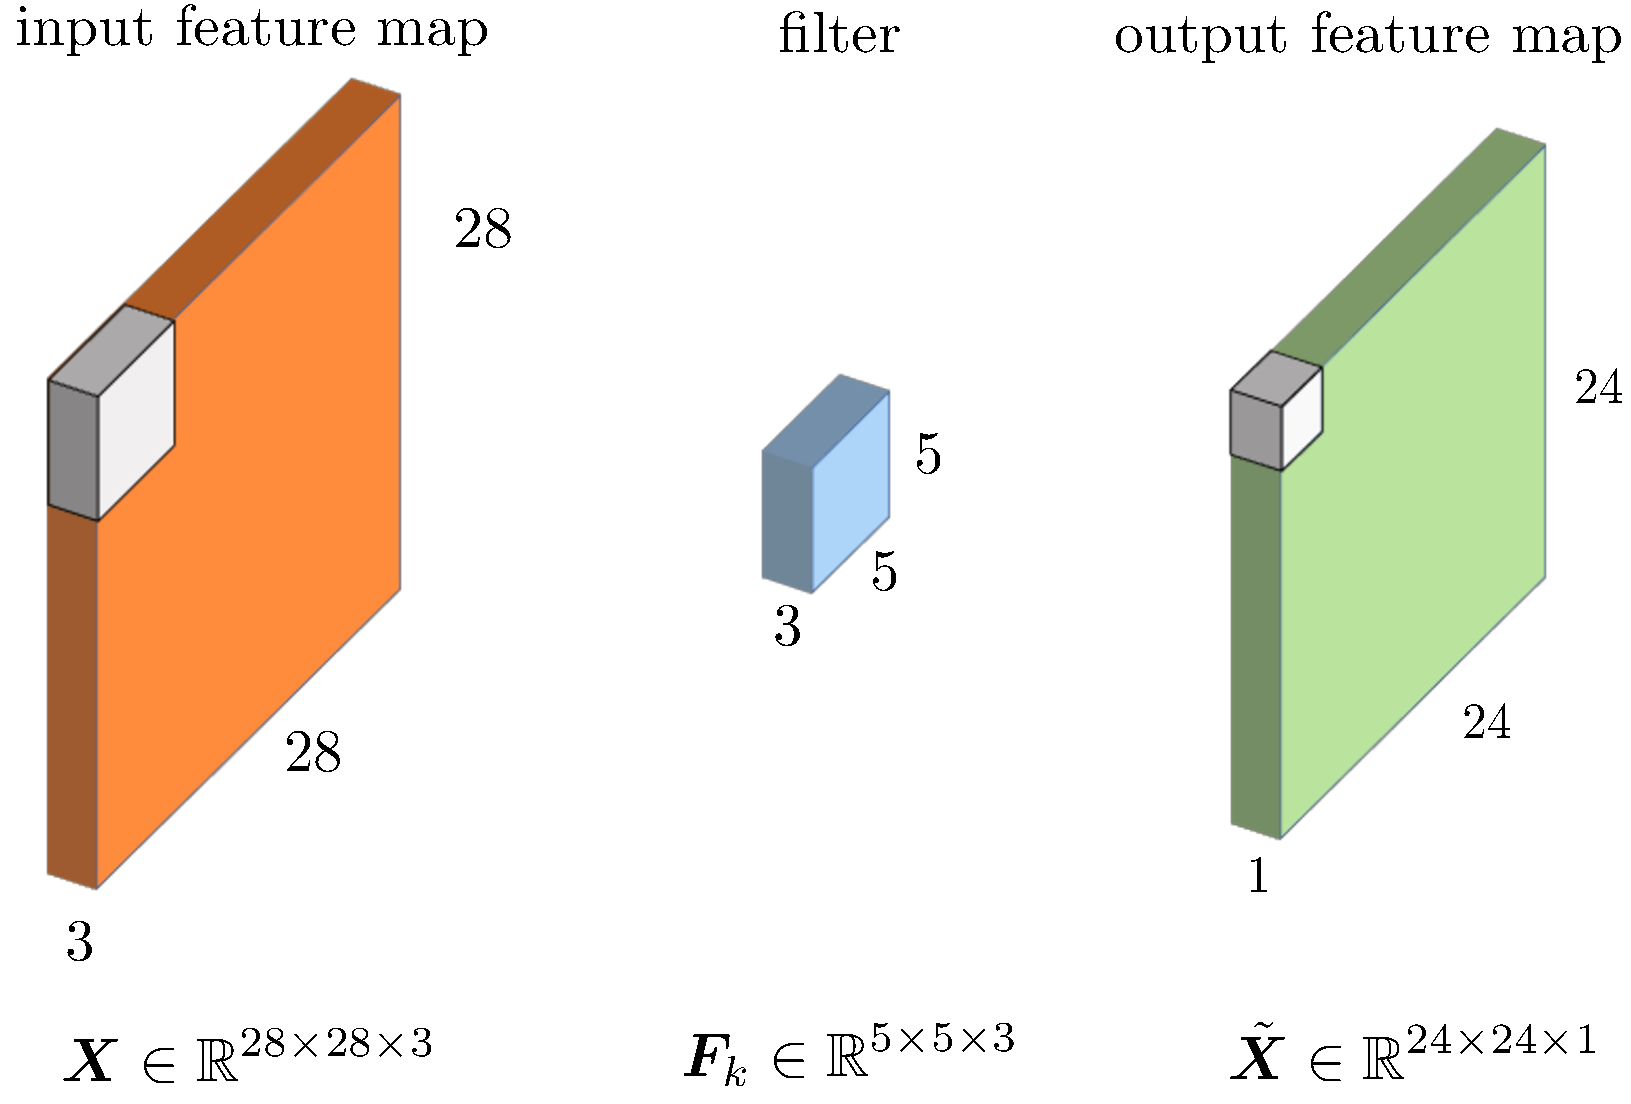
\includegraphics[height=0.4\textwidth]{convolution_3D}

\caption{$\bm{X}\in \mathbb{R}^{28\times 28 \times 3}$ represents the input feature consisting of $28 \times 28$ spatial coordinates in a total number of 3  channels / feature maps. $\bm{F}_{k}\in\mathbb{R}^{5\times 5 \times 3}$ denotes the $k$-th filter with size $5\times 5$. The third dimension $3$ of the filter automatically matches the number $3$  of channels in the previous input. Every 3D patch of $\bm{X}$ gets convolved with the filter $\bm{F}_{k}$ and this as a whole results in a single output feature map $\tilde{X}_{:,:,k}$ with size $24\times 24\times 1$. Stacking the outputs of all the filters $\{\bm{F}_{k}\}_{1\leq k\leq K}$ will lead to the output feature with size $24\times 24\times K$. \label{fig:Convolution-operation}}

\end{figure}
The outputs of convolutional layers are then followed by nonlinear activation functions. In the ReLU case, we have
\begin{equation}\label{eq:relu}
\tilde{X}_{ijk} = \sigma(O_{ijk}), \qquad \forall\, i \in [d_1-w+1], j \in [d_2-w+1], k \in [\tilde d_3].
\end{equation}
The convolution operation \eqref{eq:conv} and the ReLU activation \eqref{eq:relu} work together to extract features $\tilde{\bm{X}}$ from the input $\bm{X}$. %, which functions in a way similar to the feedforward neural net \eqref{eq:fc}.
Different from feed-forward neural nets, the filters $\bm{F}_k$ are shared across all locations $(i,j)$. A patch $[\bm{X}]_{ij}$ of an input responds strongly (that is, producing a large value) to a filter $\bm{F}_{k}$ if they are positively correlated. Therefore intuitively, each filter $\bm{F}_{k}$ serves to extract features similar to $\bm{F}_{k}$.

As a side note, after the convolution~(\ref{eq:conv}), the spatial size $d_1 \times d_2$ of the input $\bm{X}$ shrinks to ${(d_1-w+1)\times (d_2-w+1)}$ of $\tilde{\bm{X}}$. However one may want the spatial size unchanged. This can be achieved via \emph{padding}, where one appends zeros to the margins of the input $\bm{X}$ to enlarge the spatial size to $(d_1+w-1) \times (d_2+w-1)$. %The case when we apply padding to leave the spatial size unchanged is often called \emph{same convolution}, while the case with no padding is dubbed as \emph{valid convolution}. 
In addition, a \emph{stride} in the convolutional layer determines the gap $i' - i$ and $j'-j$ between two patches $\bm{X}_{ij}$ and $\bm{X}_{i'j'}$: in \eqref{eq:conv} the stride is $1$, and a larger stride would lead to feature maps with smaller sizes.

\item \emph{Pooling layer (POOL)}. A pooling layer aggregates the information of nearby features into a single one. This downsampling operation reduces the size of the features for subsequent layers and saves computation. One common form of the pooling layer is composed of the $2 \times 2$ max-pooling filter. It computes $\max \{X_{i,j,k}, X_{i+1,j,k}, X_{i,j+1,k}, X_{i+1,j+1,k} \}$, that is, the maximum of the $2 \times 2$ neighborhood in the spatial coordinates; see Figure \ref{fig:pooling} for an illustration. Note that the pooling operation is done separately for each feature map $k$. As a consequence, a $2 \times 2$ max-pooling filter acting on $\bm{X}\in \mathbb{R}^{d_1 \times d_2 \times d_3}$ will result in an output of size $d_1/2 \times d_2/2 \times d_3$. In addition, the pooling layer does not involve any parameters to optimize. Pooling layers serve to reduce redundancy since a small neighborhood around a location $(i,j)$ in a feature map is likely to contain the same information.
\end{enumerate}

\begin{figure}
\centering

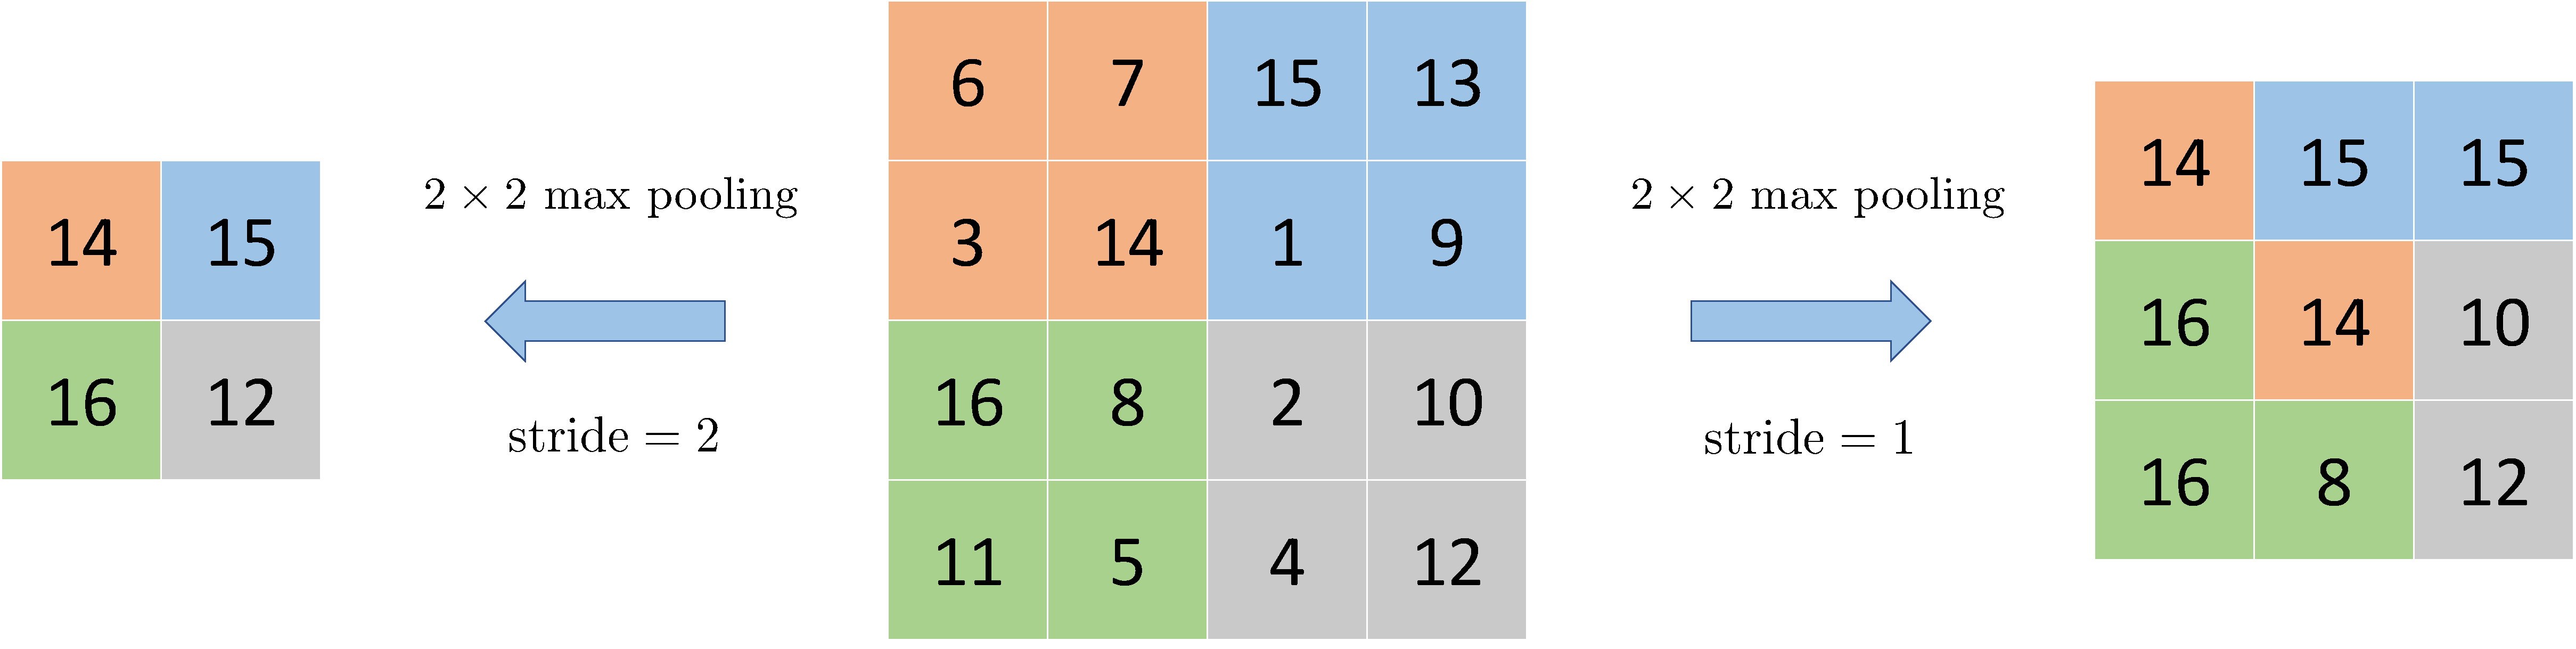
\includegraphics[width=0.95 \linewidth]{pooling}\caption{A $2\times 2$ max pooling layer extracts the maximum of 2 by 2 neighboring pixels$\,$/$\,$features across the spatial dimension. }\label{fig:pooling}
\end{figure}

In addition, we also use fully-connected layers as building blocks, which we have already seen in Section~\ref{sec:super}. Each fully-connected layer treats input tensor $\bm{X}$ as a vector $\vect(\bm{X})$, and computes $\tilde{\bm{X}} = \bsigma(\bW \vect(\bm{X}))$. A fully-connected layer does not use weight sharing and is often used in the last few layers of a CNN. As an example, Figure~\ref{fig:CNN} depicts the well-known LeNet 5 \citep{lecun1998gradient}, which is composed of two sets of CONV-POOL layers and three fully-connected layers.

%Now we are ready to build a convolutional neural network, which is simply a stack of convolutional layers, pooling layers and fully-connected layers. See 

%\begin{python}
%from keras.datasets import mnist
%from keras.models import Sequential
%from keras.layers import Dense, Flatten
%from keras.layers import Conv2D, MaxPooling2D
%
%# input image dimensions
%img_rows, img_cols = 28, 28
%
%# the data, split between train and test sets
%(x_train, y_train), (x_test, y_test) = mnist.load_data()
%x_train = x_train.reshape(x_train.shape[0], img_rows, img_cols, 1)
%x_test = x_test.reshape(x_test.shape[0], img_rows, img_cols, 1)
%input_shape = (img_rows, img_cols, 1)
%
%x_train = x_train.astype('float32')
%x_test = x_test.astype('float32')
%x_train, x_test = x_train / 255.0, x_test / 255.0
%
%LeNet = Sequential([
%    Conv2D(6, kernel_size=(5, 5), activation='relu',
%    	 padding='same', input_shape=input_shape),
%    MaxPooling2D(pool_size=(2, 2)),
%    Conv2D(16, (5, 5), activation='relu'),
%    MaxPooling2D(pool_size=(2, 2)),
%    Flatten(),
%    Dense(120, activation='relu'),
%    Dense(84, activation='relu'),
%    Dense(10, activation='softmax')]
%)
%
%LeNet.compile(loss='sparse_categorical_crossentropy',
%	optimizer='sgd', metrics=['accuracy'])
%
%history = LeNet.fit(x_train, y_train, batch_size=32, epochs=5, validation_split=0.1)
%
%score = model.evaluate(x_test, y_test, verbose=0)
%
%print('Test loss:', score[0])
%print('Test accuracy:', score[1])
%\end{python}

\begin{figure}
\centering
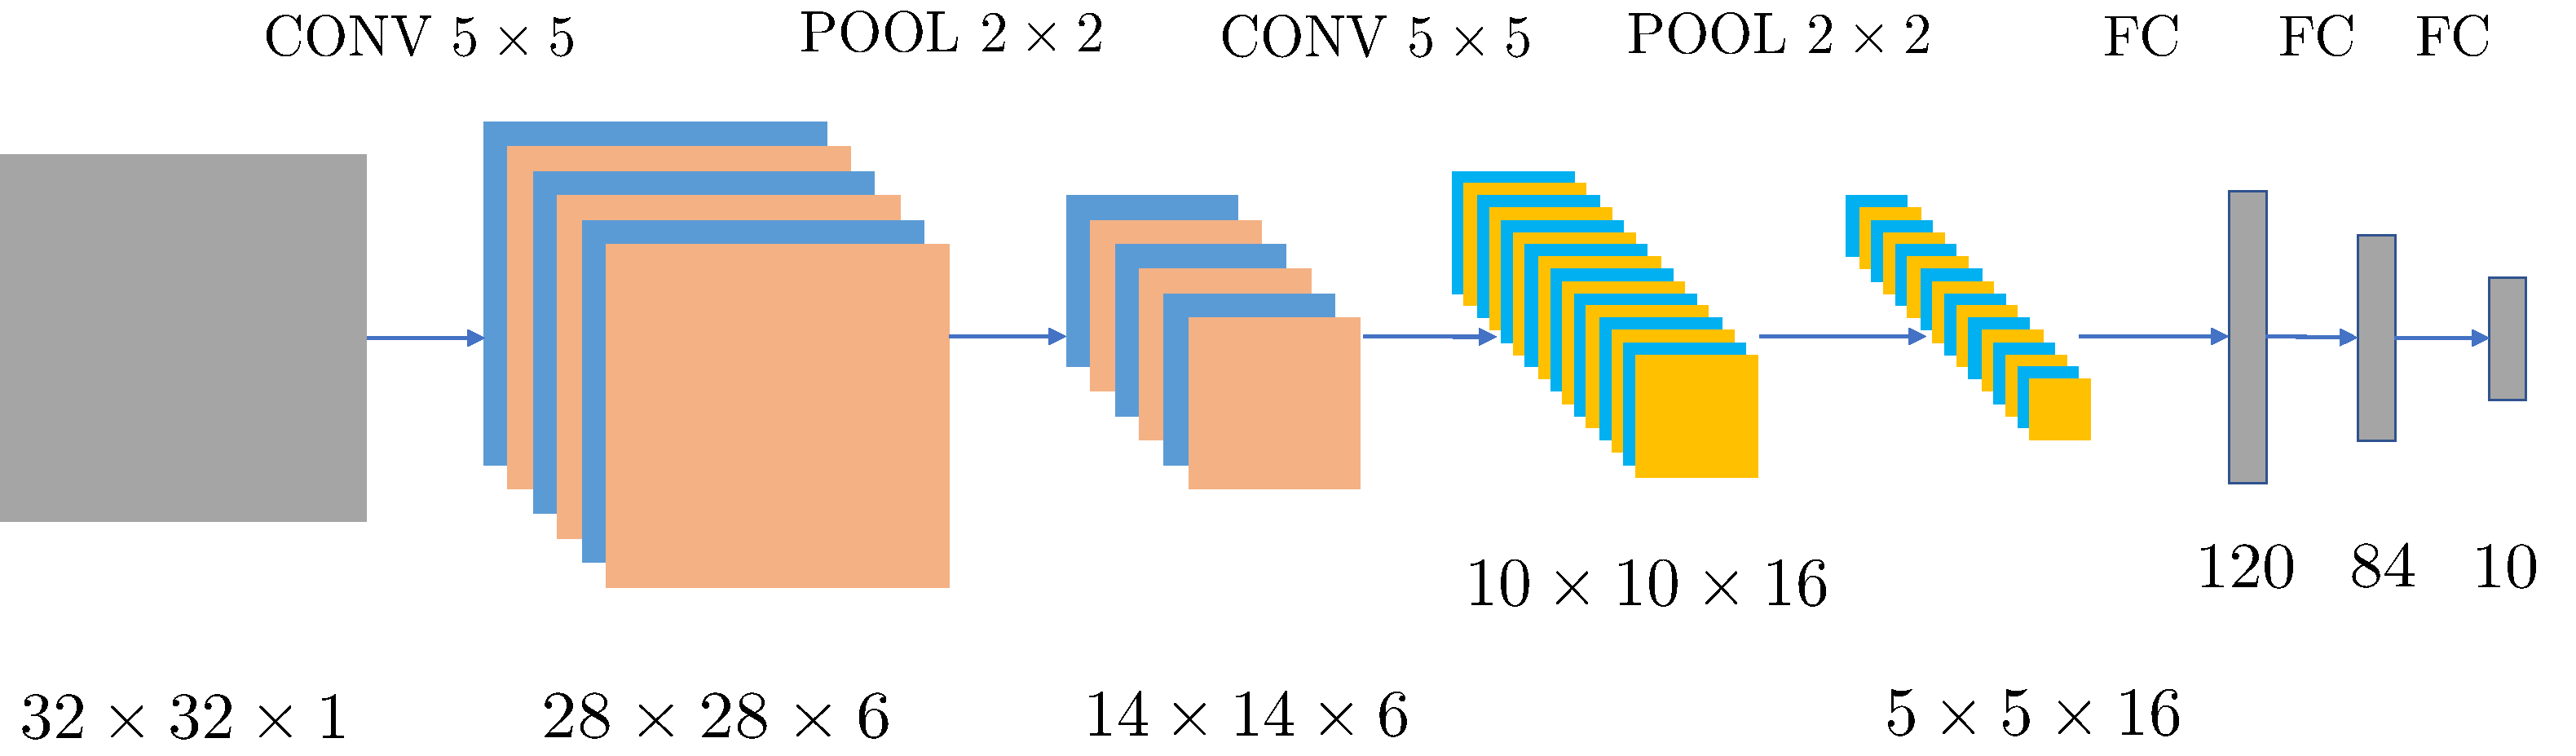
\includegraphics[width=0.9 \textwidth]{LeNet}\caption{LeNet is composed of an input layer, two convolutional layers, two pooling layers and three fully-connected layers. Both convolutions are valid and use filters with size $5 \times 5$. In addition, the two pooling layers use $2 \times 2$ average pooling. \label{fig:CNN}}
\end{figure}

